\documentclass[border=2pt]{standalone}
\usepackage{pgfplots}\pgfplotsset{compat=1.17}
\begin{document}
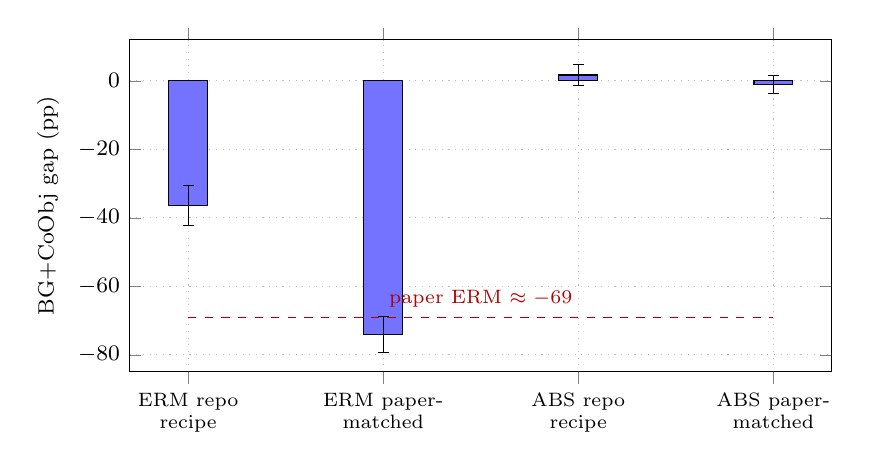
\begin{tikzpicture}
\begin{axis}[width=10.5cm,height=5.8cm,ybar,bar width=14pt,ylabel={BG+CoObj gap (pp)},symbolic x coords={ERM repo recipe,ERM paper-matched,ABS repo recipe,ABS paper-matched},xtick=data,
 x tick label style={font=\scriptsize,align=center,text width=2cm},ymin=-85,ymax=12,grid=major,grid style={dotted,gray!50},
 tick label style={font=\footnotesize},label style={font=\footnotesize}]
\addplot[fill=blue!55,error bars/.cd,y dir=both,y explicit] coordinates {(ERM repo recipe,-36.35) +- (0,5.9) (ERM paper-matched,-74.06) +- (0,5.2) (ABS repo recipe,1.71) +- (0,3.1) (ABS paper-matched,-1.03) +- (0,2.6)};
\draw[dashed,red!70!black] (axis cs:ERM repo recipe,-69) -- (axis cs:ABS paper-matched,-69) node[pos=0.5,above,font=\scriptsize,red!70!black]{paper ERM $\approx -69$};
\end{axis}
\end{tikzpicture}
\end{document}
